\documentclass[xetex,mathserif,serif]{beamer} % paused figuires for presentation
%\documentclass[handout,xetex,mathserif,serif]{beamer}% for non-paused figures
\usetheme{Singapore}
\usecolortheme{orchid}

\usepackage{amsmath} % assumes amsmath package installed
\usepackage{url}
\usepackage{epsfig}

\title[L1] % (optional, only for long titles)
{L1: Introduction}
\subtitle{Perception in Robotics, Term 3, 2020}
\author % (optional, for multiple authors)
{Gonzalo Ferrer%\inst{1}
}
\institute[Skoltech] % (optional)
{
  %\inst{1}%
  Skolkovo Institute of Science and Technology
}
\date % (optional)
{February 3, 2020}



\begin{document}

\frame{\titlepage}


\begin{frame}
\frametitle{Presentation: Who are we?}

\begin{tabular}{ l l }
  {\bf Instructor}: & Prof. Ferrer (Gonzalo)  \\
            & g.ferrer@skoltech.ru \\
  {\bf Teaching Assistants}: & Marsel Faizullin  \\
  & marsel.faizullin@skoltech.ru \\
   & Anastasia Kishkun  \\
   & anastasia.kishkun@skoltech.ru 
\end{tabular}

\vspace{5mm}

{\bf Mobile Robotics Lab}: Research group inside CDISE, it is focused on robot navigation, particularly our interests are within Path Planning and Perception and how to combine both into new solutions for robotics.

\end{frame}



% ----------------------------------------------------------------------------------
% what it is about?
% ----------------------------------------------------------------------------------
\begin{frame}
\frametitle{What is this course about?}


{\bf Why are you here? What are your expectations?}

\pause 
\vspace{5mm}

Definition of {\em Perception}:

``Awareness of something through the senses''



\begin{itemize}
\item Representation/Structure of the world: {\bf State}
\item Senses or {\bf Observations} obtained from sensors: \{Camera, Lidar, IMU, etc \}
\item Both representation must be meaningful for algorithms.
\end{itemize}

\pause
\centering
$x \in X$, (State)
 
\centering
$z \in Z$, (Observation)

\pause
\vspace{2mm}
Examples of state variables: Sensor poses, landmarks positions, map, room temperature, etc.

\end{frame}


% ----------------------------------------------------------------------------------
% Problem statement
% ----------------------------------------------------------------------------------
\begin{frame}
\frametitle{Problem Statement}

Robot (blue triangle) perceives the world, but {\em where it is??}
\begin{center}
\includegraphics[width=.5\textwidth]{localization0}
\end{center}



\pause

{\centering
The solution is a distribution of the state variables $P(x)$
}

All methods described in this course are derived following a probabilistic approach. The world is uncertain.

\end{frame}




% ----------------------------------------------------------------------------------
% Problem statement Localization
% ----------------------------------------------------------------------------------
\begin{frame}
\frametitle{Problem statement: Localization}


$P(x_1 | l_1,l_2,l_3)$

\begin{center}
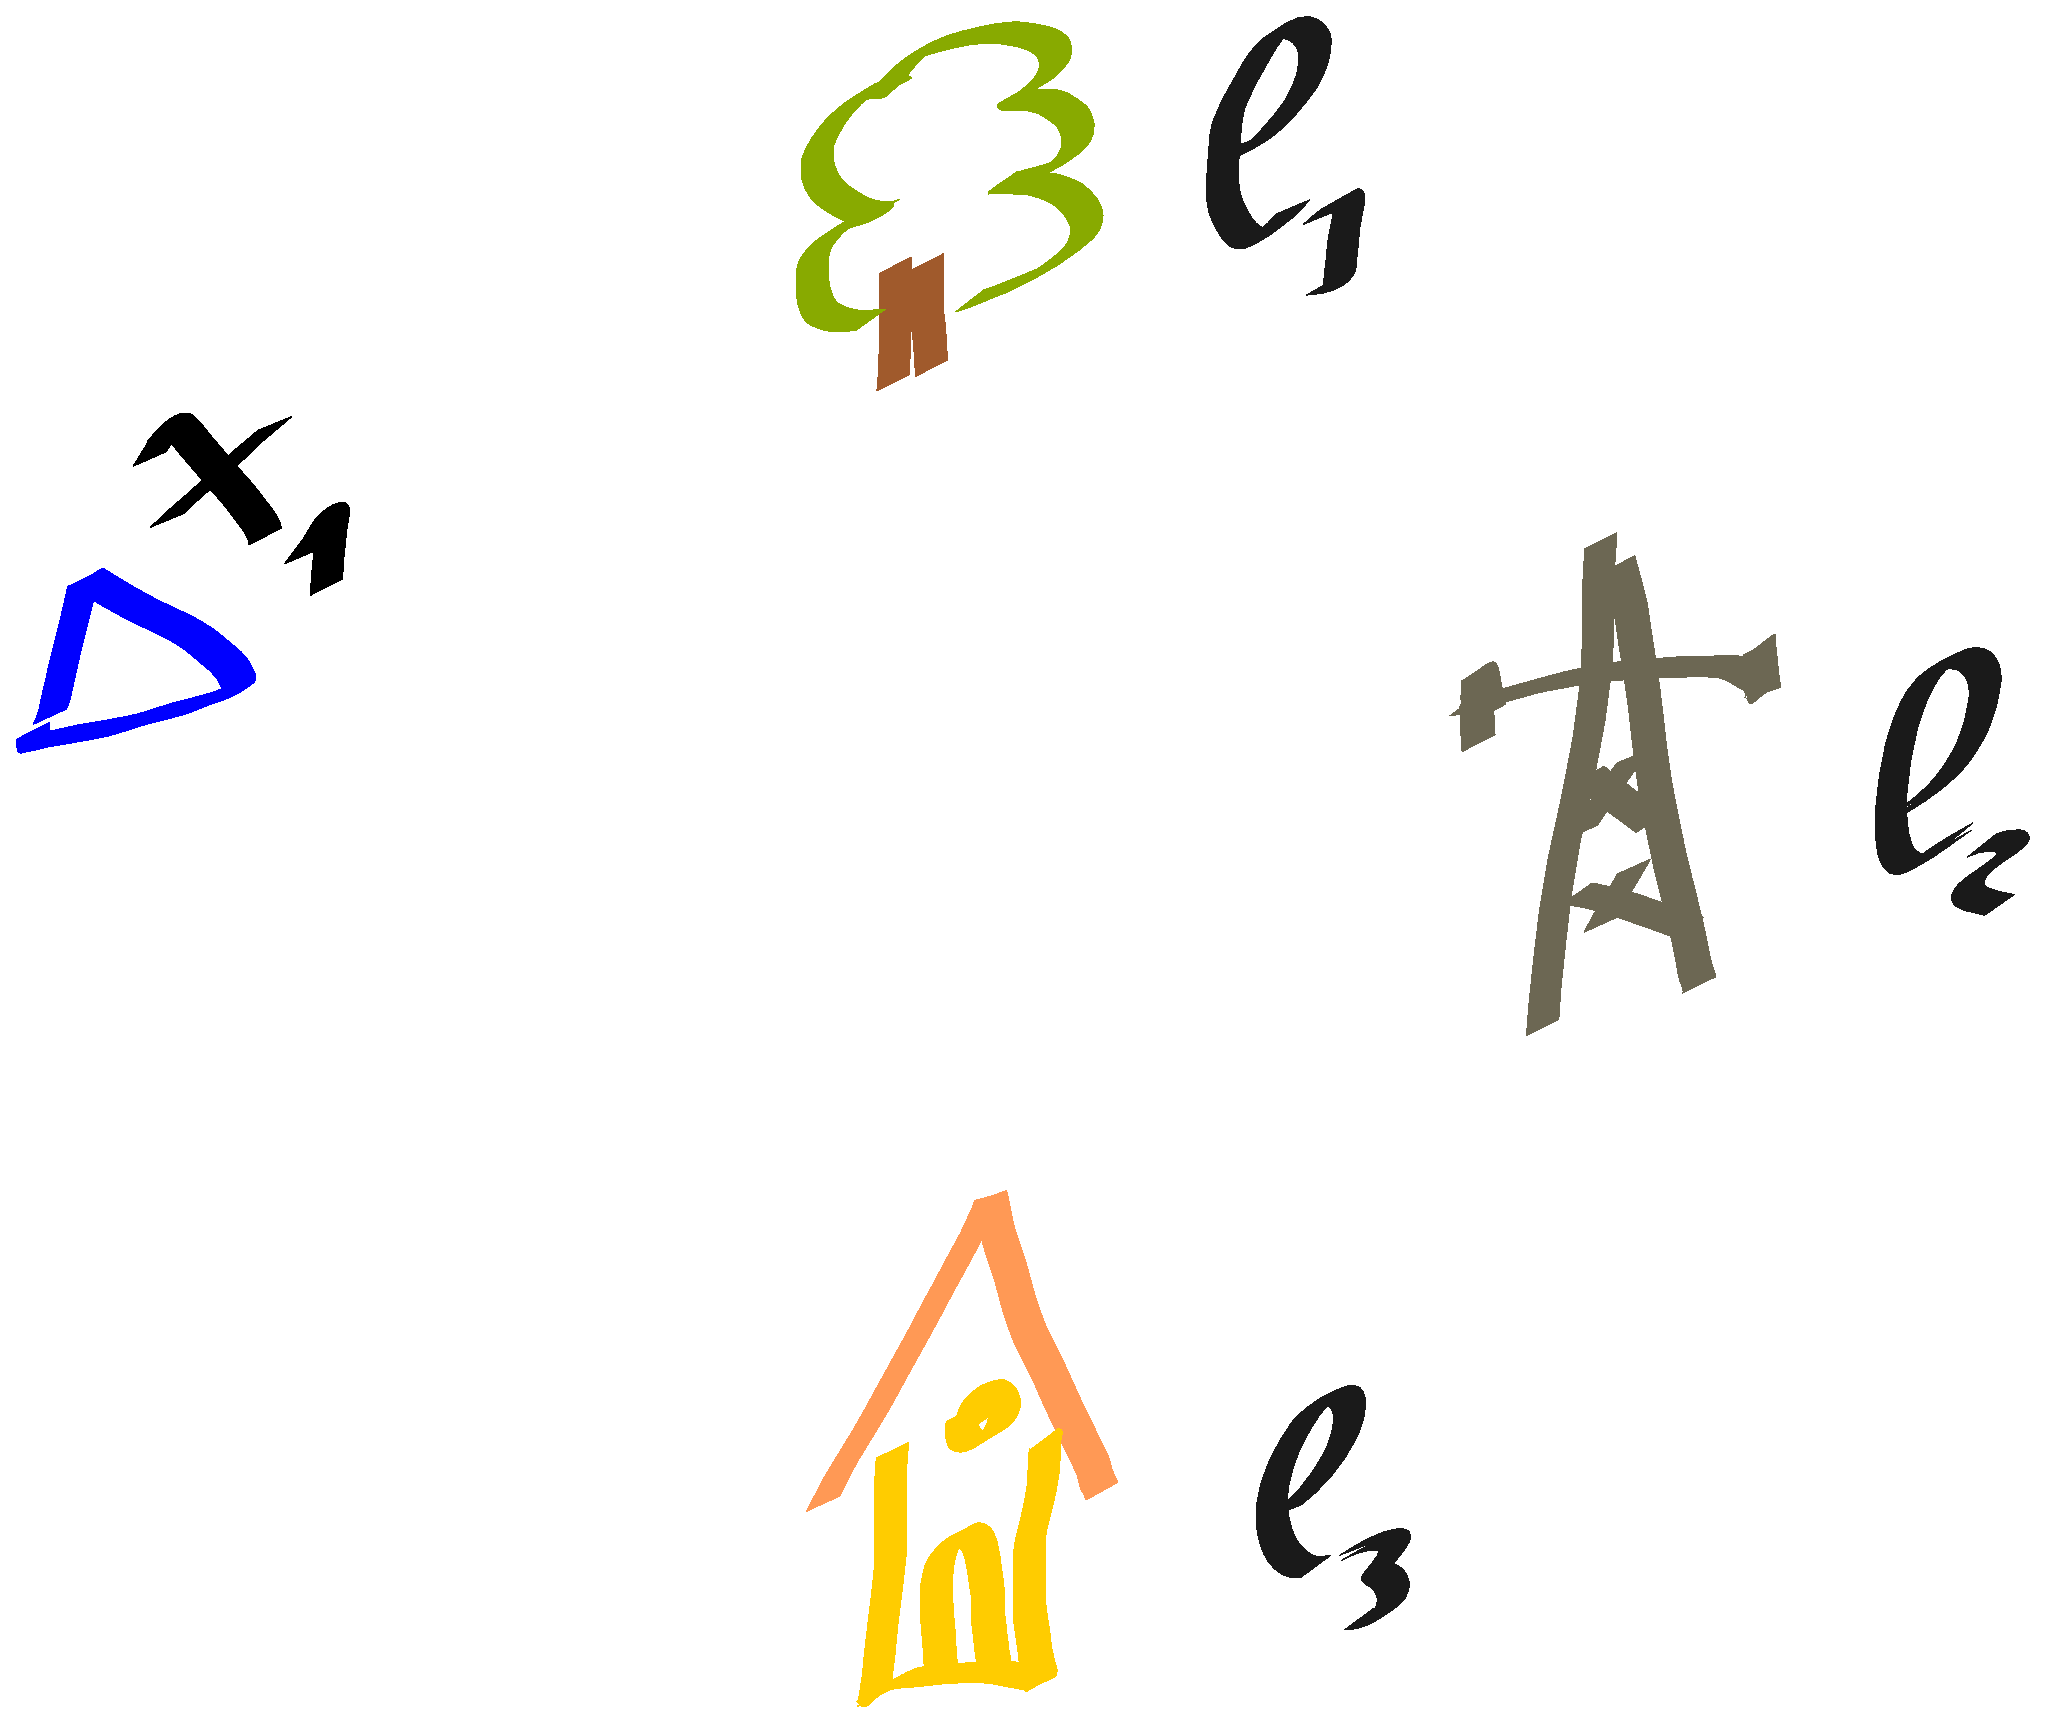
\includegraphics[width=.5\textwidth]{localization1}
\end{center}

State $x_1$ is a 2D pose (in this example) we want to estimate.

Landmarks $\{l_1,l_2,l_3\}$ are {\bf known} positions corresponding to relevant features.

\end{frame}

% ----------------------------------------------------------------------------------
% Problem statement Mapping
% ----------------------------------------------------------------------------------
\begin{frame}
\frametitle{Problem statement: Mapping}



$P(l_1,l_2,l_3 | x_1, x_2, x_3)$

\begin{center}

\includegraphics[width=.5\textwidth]{localization}
\end{center}

The opposite problem: States $\{x_1,x_2,x_3\}$ are known and landmarks $\{l_1,l_2,l_3\}$ are estimated from these known positions. 

\end{frame}

% ----------------------------------------------------------------------------------
% Problem statement SLAM
% ----------------------------------------------------------------------------------
\begin{frame}
\frametitle{Simultaneous Localization and Mapping}

\begin{center}

\includegraphics[width=.5\textwidth]{localization}
\end{center}


$P(l_1,l_2,l_3, x_1, x_2, x_3)$

\pause
The egg and the chicken problem!!

\end{frame}

% ----------------------------------------------------------------------------------
% Goals
% ----------------------------------------------------------------------------------
\begin{frame}
\frametitle{Course Goals}

\begin{itemize}
\item Mastering ( $\neq$ surveying) a set of core algorithms.
\item Development of new technologies around modern state estimation techniques.
\item Research in any field requiring precise state estimation.
\end{itemize}

\pause
\vspace{5mm}
\begin{center}
{\bf Prerequisites}
\end{center}

\begin{itemize}
\item Basic programming skills (Python)
\item Probability: there is a document in canvas, L1.5
\item Lin. Algebra: familiar with Geometry, $Ax=b$, Spectral decomp.
\end{itemize}


\end{frame}

% ----------------------------------------------------------------------------------
% Class structure
% ----------------------------------------------------------------------------------
\begin{frame}
\frametitle{Class structure}

\begin{tabular}{ l l }
  16 lectures & Monday  16:00-19:00  \\
  (B2-3007)   & Tuesday 16:00-19:00 \\
              & Thursday 16:00-19:00 \\
              \\
  40\% Problem Sets & PS1: Probability  \\
  & PS2: Localization \\
   & PS3: SLAM  \\
   & PS4: 3D Poses\\ 
   \\
   25\% Midterm exam & (3-March-2020) \\
  25\% Final Group Project &  \\
  10\% Attendance
    
\end{tabular}

\end{frame}

% ----------------------------------------------------------------------------------
% Lectures
% ----------------------------------------------------------------------------------
\begin{frame}
\frametitle{Lectures Overview}


\begin{itemize}
\item Block I: Introduction to Probabilistic Robotics (L1-5)
\item Block II: Localization (L6-7)
\item Block III: SLAM (L8-12)
\item Block IV: Advanced topics in 3D perception (L13-16)
\end{itemize}

\pause
\vspace{5mm}
Midterm (3-3-2020) will include Blocks I, II and III. The exam will consist of a mixture of theory questions, theory-based problems and practical problems, requiring simple calculus. No laptops, calculators, phones, etc. are allowed. We allow one page double-sided, hand-written formula sheet during the exam.

\end{frame}

% ----------------------------------------------------------------------------------
% Material
% ----------------------------------------------------------------------------------
\begin{frame}
\frametitle{Course Material}

\begin{itemize}
\item Your class notes.
\item Prof. handwritten lecture notes (uploaded before classes).
\item Book: {\em Probabilistic Robotics}.
S. Thurn, W. Burgard, and D. Fox, 2010, Third Printing (correct erratas)
\item Canvas, selected papers for each lecture.
\item Github {\small\url{https://github.com/Kichkun/perception_course}}
\item Telegram \url{t.me/perc_rob}
\item YouTube {\small \url{https://www.youtube.com/playlist?list=PLRXYrdEUvBoCwKsQHJzafQYb7Nut0S2bn}}
\end{itemize}

\end{frame}


% ----------------------------------------------------------------------------------
% Problem Sets
% ----------------------------------------------------------------------------------
\begin{frame}
\frametitle{Problem Sets}

\begin{itemize}
\item 4 Problem Sets (PS) during the term, due at approximately ten days intervals. 
\item PSs will be written in Python.
\item PSs are substantial and should be worked on during the full allotted time period (each is a 10\% of your grade).
\item There will be a penalty of 15\%/day. We will allow for 1 late submission without penalty (max 1 week).
\item We will consider a late submission based on the last update on canvas.
\item Students are encouraged to discuss on PS. Copying code is forbidden. On every PS there will be a section dedicated to Acknowledgments, if any.
\end{itemize}

\end{frame}


% ----------------------------------------------------------------------------------
% Policies
% ----------------------------------------------------------------------------------
\begin{frame}
\frametitle{Course Policies}

{\bf Attendance}

We will allow up to 3 missing classes and from there grade will decrease proportional to the number of absences.


\vspace{5mm}
{\bf PS Regrade Policy}

If you believe we graded a problem-set or an exam of yours incorrectly, you can submit a regrade request no later than one week after the graded work is originally returned.

\vspace{5mm}
{\bf Academic Integrity}

Reference to Skoltech's policy (see canvas)


\end{frame}


% ----------------------------------------------------------------------------------
% FInal project
% ----------------------------------------------------------------------------------
\begin{frame}
\frametitle{Final Group Project}

\begin{itemize}
\item Topic (related to the course): Extend a state of the art algorithm, or paper reproduction or implementation on your own settings.
\item 3-5 Students / group
\item Proposal: 1 page doc. Viability of the project.
\item Progress (Optional) 3 page doc. Milestone.
\item Presentation: 12' + 3' questions
\item Paper: final project document, on a IEEE template.
\end{itemize}

\end{frame}


% ----------------------------------------------------------------------------------
% Past projects
% ----------------------------------------------------------------------------------
\begin{frame}
\frametitle{Past projects}

\begin{center}
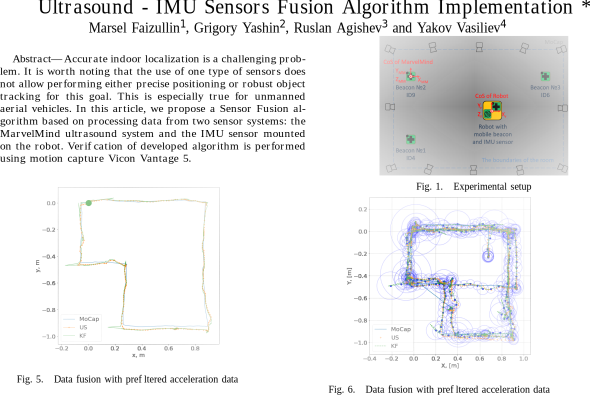
\includegraphics[width=.95\textwidth]{g1}
\end{center}

\end{frame}


% ----------------------------------------------------------------------------------
% Past projects
% ----------------------------------------------------------------------------------
\begin{frame}
\frametitle{Past projects}

\begin{center}
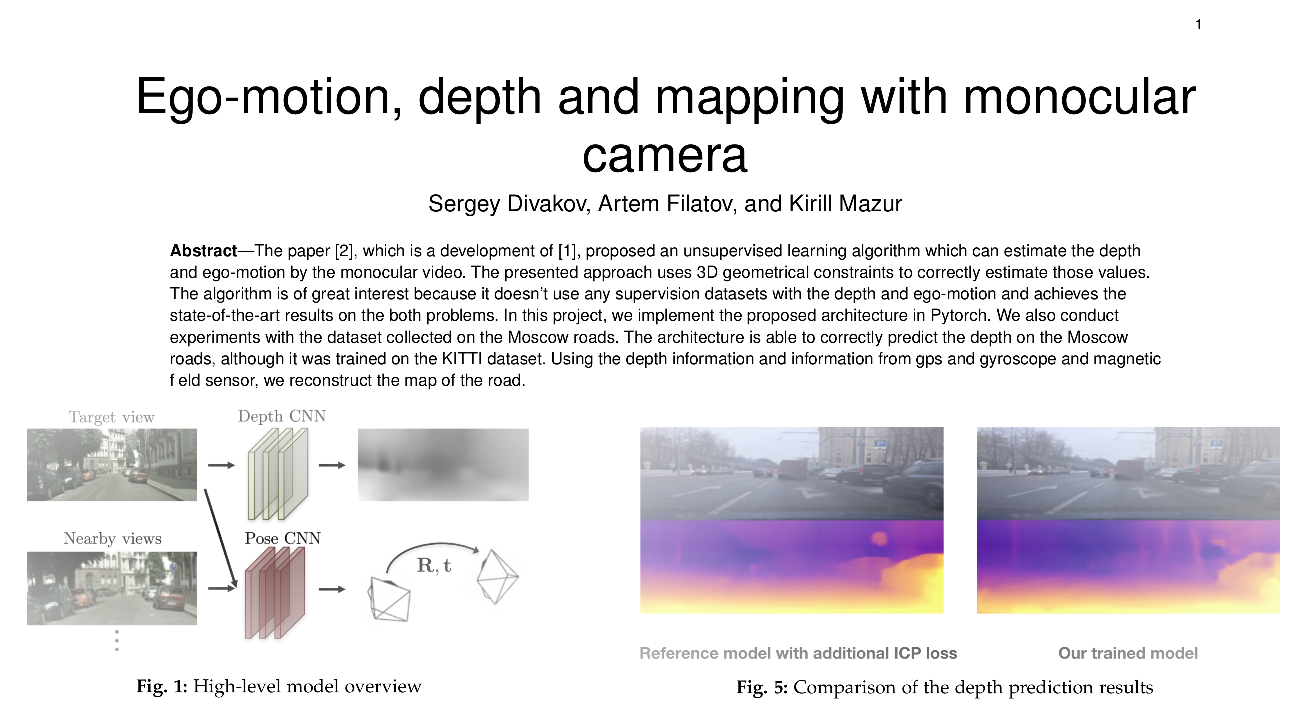
\includegraphics[width=.95\textwidth]{g2}
\end{center}

\end{frame}

% ----------------------------------------------------------------------------------
% Past projects
% ----------------------------------------------------------------------------------
\begin{frame}
\frametitle{Past projects}

\begin{center}
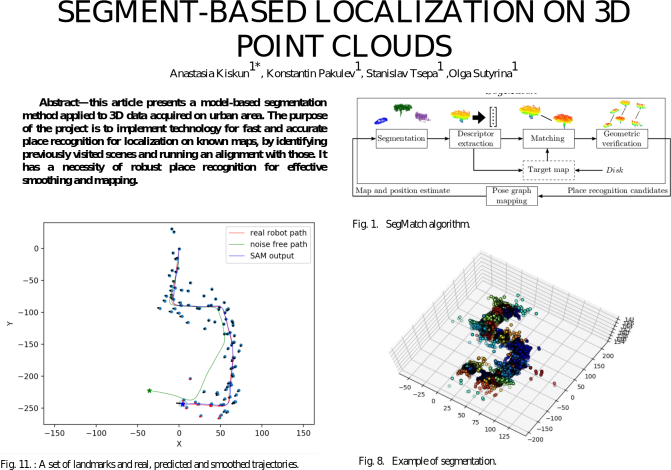
\includegraphics[width=.95\textwidth]{g3}
\end{center}

\end{frame}



% etc
\end{document}
